% !TEX root = ../main.tex
\chapter{Numerical Implementation}
\label{app:numerical_implementation}

This appendix records the numerical conventions used to obtain the results of
this thesis. The calculations use \texttt{QuTiP} for the open-system time
evolution~\cite{lambertetal2026qutip5quantum}. It documents the pulse and bath
conventions, basis ordering, operator assembly, signal construction, and
post-processing steps used throughout the thesis. Accordingly, this appendix
should be read as the numerical realisation of the spectroscopy, open-system,
and model definitions developed
in~\cref{chapter:spctr_spectroscopy,chapter:oqs_open_quantum_systems,chapter:model_systems}.

\section{Overview}
\label{app:sec:software_architecture}

Each simulation run proceeds through four stages:
\begin{enumerate}
	\item the chosen physical parameters are converted into a concrete Hamiltonian, pulse sequence, bath model, and numerical setup;
	\item for each chosen coherence time and each inhomogeneous realisation, the density matrix is propagated under the complete three-pulse sequence;
	\item the emitted third-order field is obtained by one-pulse subtraction and discrete phase cycling;
	\item the time-domain signals are averaged over disorder and Fourier transformed into the final 1D or 2D spectra.
\end{enumerate}

The physical content is therefore represented explicitly as operators, density
matrices, and time-dependent fields, while the surrounding numerical steps only
assemble and evaluate that model.

\section{Units and Time Axes}
\label{app:sec:configuration_workflow}

\subsection{Internal Units}

The transition frequencies are specified in cm$^{-1}$, but the dynamics are propagated in angular-frequency units of fs$^{-1}$. Internally the conversion is
\begin{equation}
\omega_{\mathrm{fs}^{-1}}
= 2 \pi c \cdot 10^{-5}\,\omega_{\mathrm{cm}^{-1}},
\end{equation}
with the same convention used consistently for site energies, couplings, pulse carrier frequencies, and all bath frequencies. In the code, $\hbar$ is set to unity, so Hamiltonian matrix elements are numerically expressed in the same fs$^{-1}$ units.

The bath sector is treated slightly differently. In the numerical workflow the natural control parameters are the dimensionless ratios $T/\bar{\omega}_0$, $\omega_c/\bar{\omega}_0$, and $\alpha/\bar{\omega}_0$, where
\begin{equation}
\bar{\omega}_0 = \frac{1}{N_{\mathrm{sites}}}\sum_{i=1}^{N_{\mathrm{sites}}}\omega_i.
\end{equation}
The code therefore reconstructs, for example,
\begin{equation}
T = \left(\frac{T}{\bar{\omega}_0}\right)\bar{\omega}_0,
\qquad
\omega_c = \left(\frac{\omega_c}{\bar{\omega}_0}\right)\bar{\omega}_0,
\end{equation}
before constructing the QuTiP environment. This is the same normalization used in the results chapter, where bath parameters are quoted as ratios relative to a characteristic optical scale. The choice to express bath parameters as ratios to a characteristic system scale follows the dimensionless parametrisation introduced in~\autoref{subsec:oqs_ohmic_spectral_density}.

\subsection{Time Grids and Pulse Timing}

The public detection and coherence axes always begin at zero, but the actual solver grid starts earlier because the first pulse must already be present when the propagation begins. At the numerical level, the key propagation settings introduced here are the stored output spacing \texttt{dt} and the adaptive step bound \texttt{max\_step}. The delays $t_{\mathrm{coh}}$, $t_{\mathrm{wait}}$, and $t_{\mathrm{det}}$ follow the collinear three-pulse timing convention introduced in~\autoref{fig:spctr_fwm_phase_cycling_setup} and discussed in~\autoref{sec:spctr_phase_cycling}. For a three-pulse sequence with coherence time $t_{\mathrm{coh}}$ and waiting time $t_{\mathrm{wait}}$, the pulse peaks are placed at
\begin{equation}
t_1 = -(t_{\mathrm{coh}} + t_{\mathrm{wait}}),
\qquad
t_2 = -t_{\mathrm{wait}},
\qquad
t_3 = 0.
\end{equation}
The solver-local initial time is then chosen to lie before the first pulse window. In principle this can be $-\inf$ as the system is in the thermal state, but for Gaussian pulses, the code uses
\begin{equation}
t_0 = -\Bigl(t_{\mathrm{coh}} + t_{\mathrm{wait}} + 1.823\,\tau_{\mathrm{p}}\Bigr),
\end{equation}
rounded down to the nearest multiple of the output spacing \texttt{dt}. The factor $1.823$ is the active half-width used in the laser module; at this cutoff the Gaussian intensity has already dropped below $10^{-4}$ of its peak value.

The same \texttt{dt} sets the spacing of the stored time axis, but not necessarily the adaptive solver's internal step size. Internally the adaptive upper bound \texttt{max\_step} is chosen so that the pulse envelope is sufficiently resolved when the rotating-wave approximation is used and the optical carrier is sufficiently resolved when the full laboratory-frame dynamics are propagated. Because the pulses have finite duration, this timing convention also generates the pulse-overlap regime discussed in~\autoref{subsec:results_monomer_2d_freq} and~\autoref{subsec:results_dimer_waiting_time}.

\section{Operator Representations}
\label{app:sec:model_systems}

\subsection{Basis Indexing}

The basis states defined in~\autoref{sec:model_ensemble} are stored on an
explicit ordered index set. For a model with \(N_{\mathrm{sites}}\) sites, the
ordered basis begins with the ground state, continues with the
\(N_{\mathrm{sites}}\) single-excitation states, and, when retained, appends
the double-excitation states \(\ket{ij}\) with \(i<j\). Thus the numerical
basis has the same three-band structure as in the model chapter:
\(\ket{g}\), \(\{\ket{i}\}\), and \(\{\ket{ij}\}\). Because each site is a
two-level system, \(\ket{ij}\) always denotes excitations on two different
sites. The pair states are ordered deterministically, so the mapping from a
site pair \((i,j)\) to the basis index of \(\ket{ij}\) is fixed across runs.
This is the convention that lets the same stored parameter set rebuild the same
Hamiltonian and dipole matrices reproducibly.

\subsection{Eigenbasis Transformation}

The field-free Hamiltonian and dipole operator from
~\autoref{sec:model_ensemble} are first assembled on this same ordered basis.
At this stage, the Hamiltonian is stored in the site basis, while the dipole
operator retains the adjacent-manifold structure defined in the model chapter.

The energy eigenbasis is defined by diagonalising the Hamiltonian. If $U$
denotes the resulting unitary transformation matrix, the solver-side operators
are written as
\begin{equation}
\hat{O}_{\mathrm{eig}} = U^{\dagger}\hat{O}_{\mathrm{site}}U.
\end{equation}
They are stored in the energy eigenbasis. The eigenvectors are additionally
phase-fixed numerically so that the first nonzero component of each eigenvector
is real and positive, which makes stored eigenbasis quantities reproducible
across runs.

\section{Laser Pulses and Light-Matter Interaction}
\label{app:sec:laser_field}

The pulse model stores three pulses with amplitudes $A_k$, phases $\phi_k$, common carrier frequency $\omega_L$, a chosen envelope type, and FWHM $\tau_{\mathrm{p}}$. The three-pulse field convention implemented here follows the main-text definitions of the applied field and its positive-/negative-frequency decomposition in~\cref{eq:spctr_E_three_pulses_space,eq:spctr_E_plusminus}; the only additional ingredient is the numerical truncation of the envelope to finite support. Two envelope types are implemented: Gaussian and $\cos^2$. For the Gaussian case the code evaluates
\begin{equation}
\label{eq:laser_envelope}
s_k(t)
=
\exp\!\left[
-\frac{(t-t_k)^2}{2\sigma^2}
\right],
\qquad
\sigma = \frac{\tau_{\mathrm{p}}}{2\sqrt{2\ln 2}},
\end{equation}
only inside the active time window $[t_k-1.823\tau_{\mathrm{p}},\, t_k+1.823\tau_{\mathrm{p}}]$. Inside that window the boundary value is subtracted,
\begin{equation}
s_k^{\mathrm{num}}(t) = \max\!\bigl(s_k(t)-s_k(t_k \pm 1.823\tau_{\mathrm{p}}),0\bigr),
\end{equation}
so that the pulse envelope vanishes continuously at the numerical cutoff. Outside the active window the field is set exactly to zero to enable a free field evolution.

The code distinguishes carefully between the full laboratory-frame positive-frequency field and its slowly varying envelope. Accordingly, the scalar dipole Hamiltonian of~\autoref{eq:spctr_semiclassical_hamiltonian_scalar} is implemented either with the full laboratory-frame field or, under the RWA, with the decomposition of~\autoref{eq:spctr_E_plusminus}. In the notation used internally,
\begin{equation}
\varepsilon^{(+)}(t) = e^{-i\omega_L t} E(t),
\qquad
E(t) = \sum_{k=1}^{3} A_k s_k(t)e^{-i\phi_k},
\end{equation}
where $\omega_L$ is the common carrier frequency and $\phi_k$ are the phase-cycling phases. The non-RWA implementation uses the full field $\varepsilon^{(+)}(t)$ and the full dipole operator,
\begin{equation}
H_{\mathrm{int}}(t)
=
-\hat{\mu}\Bigl(\varepsilon^{(+)}(t)+\varepsilon^{(-)}(t)\Bigr),
\end{equation}
whereas the RWA implementation uses the slowly varying envelope,
\begin{equation}
H_{\mathrm{int}}^{\mathrm{RWA}}(t)
=
-\Bigl(\hat{\mu}^{(-)}E^{*}(t)+\hat{\mu}^{(+)}E(t)\Bigr).
\label{eq:app_rwa_interaction_hamiltonian}
\end{equation}
This is the convention used both by the generic Hamiltonian treatment and by
the explicit equations of motion.

\section{Open Quantum System Terms}
\label{app:sec:oqs_evolution}

\subsection{Initial State}

The default initial state is the ground-state density matrix. For
finite-temperature Redfield calculations, the code can also construct a
Boltzmann state in the energy eigenbasis,
\begin{equation}
\rho_{\mathrm{th}}
=
\frac{1}{Z}\sum_{a} e^{-E_a/T}\ket{a}\!\bra{a},
\end{equation}
but this option is intentionally restricted to Redfield runs, because that is
the only backend for which the code treats finite-temperature equilibration
consistently. This option specialises the Gibbs-state construction
of~\autoref{eq:oqs_ho_gibbs_state} to the system eigenbasis used by the solver.

\subsection{Numerical Backend Realisation}

\todoimp{this has too be made consistent and smooth}
The operator definitions themselves are part of the physical model and were
introduced in~\cref{sec:model_ensemble}.
At the implementation level, both open-system backends first assemble these
operators on the ordered basis described above and then transform them to the
energy eigenbasis before propagation.

For Lindblad runs, the monomer uses the phenomenological relaxation and
dephasing operators.

For Bloch--Redfield runs, the same site-local operators are coupled to mutually
uncorrelated bosonic baths and passed to the QuTiP Redfield solver in the
energy eigenbasis. The bath families and spectral densities used numerically are
therefore implementations of the microscopic model introduced in
~\cref{eq:oqs_Interaction_Hamiltonian,eq:oqs_Rabcd_full}, not additional model
assumptions.


\subsection{Explicit Equations of motion}
\label{app:sec:paper_eqs_explicit_eoms}

The third option is a hard-coded implementation of the equations-of-motion form used for direct
comparison with the monomer and dimer benchmarks of~\cite{mancaletal2006twodimensionalopticalthreepulse, pisliakovetal2006twodimensionalopticalthreepulse}. 


\noindent\textbf{Monomer Equations.}

Using the rotating-frame ansatz
\begin{equation}
\rho_{eg}(t)=\sigma_{eg}(t)\,\mathrm{e}^{-\mathrm{i}\omega_L t},
\qquad
\rho_{ge}(t)=\sigma_{ge}(t)\,\mathrm{e}^{+\mathrm{i}\omega_L t},
\end{equation}
the implemented monomer equations are
\begin{align}
\dot{\sigma}_{eg}
&=
-\bigl(\Gamma + i\Delta_{L}\bigr)\sigma_{eg}
+ i\,\mu_{eg} E(t)\,\bigl(\rho_{gg}-\rho_{ee}\bigr),
\label{eq:app_monomer_eom_sigma_eg}
\\
\dot{\rho}_{ee}
&=
-\gamma_{\downarrow}\rho_{ee}
+ \gamma_{\uparrow}\rho_{gg}
+ i\,\mu_{eg}E(t)\sigma_{ge}
- i\,\mu_{eg}E^{*}(t)\sigma_{eg},
\notag
\\
\dot{\rho}_{gg}
&=
-\gamma_{\uparrow}\rho_{gg}
+ \gamma_{\downarrow}\rho_{ee}
- i\,\mu_{eg}E(t)\sigma_{ge}
+ i\,\mu_{eg}E^{*}(t)\sigma_{eg},
\label{eq:app_monomer_eom_rho_gg}
\end{align}
with
\begin{equation}
\Gamma = \gamma_{\varphi} + \frac{\gamma_{\downarrow}+\gamma_{\uparrow}}{2},
\qquad
\Delta_{L}=\omega_{eg}-\omega_L.
\end{equation}
For the monomer runs used here, \(\gamma_{\uparrow}=0\), so the equations reduce to the familiar phenomenological monomer form used in the main results chapter.

\noindent\textbf{Dimer Equations.}

For the dimer backend, the relevant dipole matrix elements are the eigenbasis couplings \(\mu_{10},\mu_{20},\mu_{31},\mu_{32}\). The level structure and adjacent-manifold dipole couplings used here are the ones introduced in~\autoref{sec:model_dimer_esa} and summarised in~\autoref{fig:rslts_dimer_basis_map}. The transition frequencies are \(\omega_{ab}=E_a-E_b\). The damping and transfer rates are not inserted phenomenologically, but are deduced from the actual Redfield tensor of the microscopic bath model introduced in~\cref{eq:oqs_Interaction_Hamiltonian,eq:oqs_Rabcd_full} and evaluated through the bath power spectrum~\cref{eq:oqs_Noise_Power_Spectrum}. The rotating-frame ansatz is
\begin{equation}
    \rho_{10}=\sigma_{10}\mathrm{e}^{-\mathrm{i}\omega_L t},
    \quad
    \rho_{20}=\sigma_{20}\mathrm{e}^{-\mathrm{i}\omega_L t},
    \quad
    \rho_{30}=\sigma_{30}\mathrm{e}^{-2\mathrm{i}\omega_L t},
    \quad
    \rho_{31}=\sigma_{31}\mathrm{e}^{-\mathrm{i}\omega_L t},
    \quad
    \rho_{32}=\sigma_{32}\mathrm{e}^{-\mathrm{i}\omega_L t},
\end{equation}
while the intraband coherence \(\rho_{12}\) and the populations \(\rho_{aa}\) are left unchanged. In this notation the implemented equations read
\begin{align}
\dot{\sigma}_{10}
&=
-\bigl[i(\omega_{10}-\omega_L)+\Gamma_{10}\bigr]\sigma_{10}
+ iE(t)\bigl[\mu_{10}(\rho_{00}-\rho_{11})-\mu_{20}\rho_{12}\bigr]
+ iE^{*}(t)\mu_{31}\sigma_{30},
\\
\dot{\sigma}_{20}
&=
-\bigl[i(\omega_{20}-\omega_L)+\Gamma_{20}\bigr]\sigma_{20}
+ iE(t)\bigl[\mu_{20}(\rho_{00}-\rho_{22})-\mu_{10}\rho_{21}\bigr]
+ iE^{*}(t)\mu_{32}\sigma_{30},
\\
\dot{\sigma}_{30}
&=
-\bigl[i(\omega_{30}-2\omega_L)+\Gamma_{30}\bigr]\sigma_{30}
+ iE(t)\bigl[\mu_{31}\sigma_{10}+\mu_{32}\sigma_{20}
- \mu_{10}\sigma_{31}-\mu_{20}\sigma_{32}\bigr],
\end{align}
\begin{align}
\dot{\sigma}_{31}
&=
-\bigl[i(\omega_{31}-\omega_L)+\Gamma_{31}\bigr]\sigma_{31}
+ iE(t)\bigl[\mu_{31}(\rho_{11}-\rho_{33})+\mu_{32}\rho_{21}\bigr]
- iE^{*}(t)\mu_{10}\sigma_{30},
\\
\dot{\sigma}_{32}
&=
-\bigl[i(\omega_{32}-\omega_L)+\Gamma_{32}\bigr]\sigma_{32}
+ iE(t)\bigl[\mu_{32}(\rho_{22}-\rho_{33})+\mu_{31}\rho_{12}\bigr]
- iE^{*}(t)\mu_{20}\sigma_{30},
\\
\dot{\rho}_{12}
&=
-\bigl(i\omega_{12}+\Gamma_{12}\bigr)\rho_{12}
+ iE(t)\bigl[\mu_{10}\sigma_{02}-\mu_{32}\sigma_{13}\bigr]
+ iE^{*}(t)\bigl[\mu_{31}\sigma_{32}-\mu_{20}\sigma_{10}\bigr],
\end{align}
\begin{align}
\dot{\rho}_{11}
&=
-\Gamma_{11}\rho_{11}
+ \gamma_{12}\rho_{22}
+ iE(t)\bigl[\mu_{10}\sigma_{01}-\mu_{31}\sigma_{13}\bigr]
+ iE^{*}(t)\bigl[\mu_{31}\sigma_{31}-\mu_{10}\sigma_{10}\bigr],
\\
\dot{\rho}_{22}
&=
-\Gamma_{22}\rho_{22}
+ \gamma_{21}\rho_{11}
+ iE(t)\bigl[\mu_{20}\sigma_{02}-\mu_{32}\sigma_{23}\bigr]
+ iE^{*}(t)\bigl[\mu_{32}\sigma_{32}-\mu_{20}\sigma_{20}\bigr],
\\
\dot{\rho}_{00}
&=
-iE(t)\bigl[\mu_{10}\sigma_{01}+\mu_{20}\sigma_{02}\bigr]
+ iE^{*}(t)\bigl[\mu_{10}\sigma_{10}+\mu_{20}\sigma_{20}\bigr].
\end{align}
The rates entering these equations can be written in terms of the dimer mixing angle
\(\theta\) from~\autoref{eq:dimer_mixing_angle} and the bath power spectrum
\(\mathcal{S}(\omega)\) as
\begin{align}
\gamma_{12} &= \sin^{2}(2\theta)\,\mathcal{S}(\omega_{21}),
\qquad
\gamma_{21} = \sin^{2}(2\theta)\,\mathcal{S}(\omega_{12}),
\\
\Gamma_{10} &= \Gamma_{31}
= \left(1-\frac{1}{2}\sin^{2}(2\theta)\right)\mathcal{S}(0)
+ \frac{\gamma_{21}}{2},
\\
\Gamma_{20} &= \Gamma_{32}
= \left(1-\frac{1}{2}\sin^{2}(2\theta)\right)\mathcal{S}(0)
+ \frac{\gamma_{12}}{2},
\\
\Gamma_{30} &= 2\mathcal{S}(0),
\qquad
\Gamma_{12} = 2\cos^{2}(2\theta)\,\mathcal{S}(0)
+ \frac{\gamma_{12}+\gamma_{21}}{2},
\\
\Gamma_{11} &= \gamma_{21},
\qquad
\Gamma_{22} = \gamma_{12}.
\end{align}
This is exactly the Appendix-C form used for the hard-coded dimer benchmark equations in
Paper~II, but here written explicitly in terms of the underlying Redfield rates instead of
leaving the \(\Gamma_{ij}\) implicit.

The remaining equations are fixed by Hermiticity and normalization:
\begin{equation}
\rho_{21}=\rho_{12}^{*},
\qquad
\sigma_{01}=\sigma_{10}^{*},
\qquad
\sigma_{02}=\sigma_{20}^{*},
\qquad
\sigma_{13}=\sigma_{31}^{*},
\qquad
\sigma_{23}=\sigma_{32}^{*},
\qquad
\dot{\rho}_{33}=-\dot{\rho}_{00}-\dot{\rho}_{11}-\dot{\rho}_{22}.
\end{equation}

This explicit $16\times 16$ construction also clarifies one point where the present implementation is more explicit than Paper~II. In the printed appendix there, only the subset of equations labelled (D1)--(D6) is written out and the elements involving the second one-exciton state are then generated by the substitution \(1\leftrightarrow 2\). However, when the full RWA commutator is reconstructed in Liouville space, the coherences \(\sigma_{31}\) and \(\sigma_{32}\) also contain terms proportional to the upper-manifold population \(\rho_{33}\). In other words, the full commutator structure yields the combinations
\begin{equation}
iE(t)\bigl[\mu_{31}(\rho_{11}-\rho_{33})+\mu_{32}\rho_{21}\bigr],
\qquad
iE(t)\bigl[\mu_{32}(\rho_{22}-\rho_{33})+\mu_{31}\rho_{12}\bigr],
\end{equation}
not only the lower-state pieces proportional to \(\mu_{31}\rho_{11}\) and \(\mu_{32}\rho_{22}\). These \(\rho_{33}\)-terms are not written explicitly in the printed appendix of Paper~II, but they are required by the same commutator that generates the rest of the Liouvillian and by consistency with the trace-preserving population equation. The implementation therefore keeps the completed form of the dimer equations rather than a literal transcription of the shortened printed list.

\subsection{Solver Diagnostics and Time Cutoff}

Because the Redfield equation can lead to unphysical density matrices, before a simulation is launched, the workflow runs a dedicated diagnostic. The code uses the maximal configured coherence time \(t_{\mathrm{coh,max}}\), fixes the three pulse phases to \((\phi_1,\phi_2,\phi_3)=(0,0,0)\), propagates one full trajectory, and checks at every stored time point whether the density matrix remains Hermitian, trace preserving, and positive semidefinite. The positivity test is not performed with exact arithmetic, with a numerical threshold of
\begin{equation}
\lambda_{\min}(\rho(t)) \ge -10^{-6},
\end{equation}
where \(\lambda_{\min}\) denotes the smallest eigenvalue of the propagated density matrix. The first time at which Hermiticity, positivity, or trace preservation fails defines a numerical cutoff time \(t_{\mathrm{cut}}\). The emitted field is then multiplied by a mask that sets the signal to zero for \(t_{\mathrm{det}} > t_{\mathrm{cut}}\). While it doesnt guarantee, that every possible trajectory remains physical, this is an important safeguard.

The role of this check is best understood as a worst-case preflight test for the whole batch, not as a diagnostic repeated independently for every phase-cycling combination. Once a configuration has passed at \(t_{\mathrm{coh,max}}\), the resulting \(t_{\mathrm{cut}}\) is stored in the job metadata and reused during the full signal-construction workflow. For the regenerated dimer comparison figures promoted into the main text, the stored metadata give \(t_{\mathrm{cut}}=\infty\), so the published thesis figures are not additionally truncated by this safeguard. If the diagnostic were to fail, however, the cutoff would be enforced automatically in the emitted-field construction before the Fourier transform is taken.

The same trajectory-level analysis is also useful for quantifying how much secularization changes an otherwise fixed Redfield simulation. The approximation being tested here is precisely the secularization discussed in~\autoref{subsec:oqs_Fourier_and_secular}. For two arbitrary density operators \(\rho\) and \(\sigma\), the trace distance is defined as
\begin{equation}
D_{\mathrm{tr}}(\rho,\sigma)
=
\frac{1}{2}\left\|\rho-\sigma\right\|_1,
\end{equation}
with trace norm
\begin{equation}
\|A\|_1 = \mathrm{Tr}\sqrt{A^{\dagger}A}.
\end{equation}
In \autoref{fig:app_dimer_redfield_sec_cutoff_diagnostic}, the physical parameters are chosen to match the coupled dimer discussed in~\autoref{subsec:results_dimer_coupled_case}; only the dissipative treatment is switched between full Bloch--Redfield and secular Bloch--Redfield, and the stored output spacing is refined from \(\Delta t=\SI{2}{\femto\second}\) to \(\Delta t=\SI{1}{\femto\second}\) so that the driven evolution is resolved more clearly. Denoting the two trajectories by \(\rho_{\mathrm{full}}(t)\) and \(\rho_{\mathrm{sec}}(t)\), the pointwise comparison is \(D_{\mathrm{tr}}(\rho_{\mathrm{full}}(t),\rho_{\mathrm{sec}}(t))\). To summarize the full trajectory in two numbers, define
\begin{equation}
D_{\max} = \max_t D_{\mathrm{tr}}(\rho_{\mathrm{full}}(t),\rho_{\mathrm{sec}}(t)),
\qquad
D_{\mathrm{mean}} =
\frac{1}{t_f-t_i}\int_{t_i}^{t_f}
D_{\mathrm{tr}}(\rho_{\mathrm{full}}(t),\rho_{\mathrm{sec}}(t))\,dt.
\end{equation}
For the present pulse-driven coupled dimer trajectory, this gives \(D_{\max}=3.03\times10^{-2}\) at \(t=\SI{17}{\femto\second}\) and \(D_{\mathrm{mean}}=2.26\times10^{-2}\) over the stored solver-local trajectory. The largest matrix-element change occurs in the ground-state population \(\rho_{00}\), for which \(\max_t |\Delta\rho_{00}(t)| = 3.02\times10^{-2}\). Thus, for this coupled dimer the secular approximation changes the driven evolution at a clearly visible few-percent level, while the positivity diagnostic still remains safely above the numerical threshold and yields \(t_{\mathrm{cut}}=\infty\) for both propagators.

\begin{figure}[htbp]
    \centering
    \safeplaceholdergraphic[0.98\linewidth]{figures/app_dimer_redfield_sec_cutoff_diagnostic}
    \caption{Numerical diagnostic for secularization in the coupled dimer. Top: the largest density-matrix difference between the full Bloch--Redfield and secular Bloch--Redfield trajectories appears in \(|\rho_{00}(t)|\). Middle: the corresponding whole-state difference, quantified by the trace distance \(D_{\mathrm{tr}}\). Bottom: the workflow positivity diagnostic at \((\phi_1,\phi_2,\phi_3)=(0,0,0)\). In both cases the minimum eigenvalue stays above the threshold \(\lambda_{\min}\ge -10^{-6}\), so the stored cutoff time is \(t_{\mathrm{cut}}=\infty\).}
    \label{fig:app_dimer_redfield_sec_cutoff_diagnostic}
\end{figure}

\section{Construction of the Third-Order Signal}
\label{app:sec:third_order_polarisation}

\subsection{Positive-Frequency Polarisation}

After propagation, the emitted signal is extracted from the density matrix through the positive-frequency part of the dipole operator,
\begin{equation}
P^{(+)}(t) = \mathrm{Tr}\!\left[\hat{\mu}^{(+)}\rho(t)\right].
\end{equation}
This is the implementation of the microscopic dipole expectation value from~\autoref{eq:spctr_P_def_spectroscopy}, restricted to the radiating positive-frequency component relevant for the emitted-field relation~\autoref{eq:spctr_signal_field_from_polarisation}.
In the actual implementation, $\hat{\mu}^{(+)}$ is obtained by taking the strictly lower-triangular part of the dipole matrix in the ordered eigenbasis. This keeps only the radiating transitions from lower to higher excitation sectors in the convention adopted by the code. The result is a complex signal, so both amplitude and phase are retained explicitly throughout the pipeline.

The solver-local trajectory is generally longer than the public detection window. The code therefore computes the full propagated polarisation and then slices it back onto the public detection axis $t_{\mathrm{det}} \in [0,T_{\mathrm{det}}]$. This keeps the pulse action and the subsequent free evolution on one continuous internal grid while ensuring that all saved artefacts use the same detection axis.

\subsection{One-Pulse Subtraction}

The thesis implementation uses a non-perturbative three-pulse propagation, but the desired observable is still the third-order response. To isolate it numerically, the code evaluates, for every phase setting, one run with all three pulses present and three auxiliary runs in which only a single pulse is active. The background-subtracted signal is then
\begin{equation}
P^{(3)}(t)
\approx
P_{\mathrm{total}}(t)
- P_{(1)}(t)
- P_{(2)}(t)
- P_{(3)}(t),
\label{eq:third_order_signal_numerical}
\end{equation}
which is the implemented form of third-order isolation in the weak-field regime. In the thesis calculations, the pulse amplitudes are chosen weak enough that higher-order contamination remains numerically negligible.
In weak fields, this subtraction is the numerical counterpart of isolating the third-order contribution \(P^{(3)}\) in~\autoref{eq:spctr_P3_convolution_thesis} from the full driven response.

\subsection{Discrete Phase Cycling}

For a given coherence time and a given disorder realisation, the code evaluates the phase grid. Here $n_{\phi}$ denotes the number of sampled carrier phases per pulse, so that the numerical phase-cycling resolution is fixed by the chosen phase grid. This discrete Fourier sum is the finite-grid realisation of the carrier-phase projection derived in~\autoref{eq:spctr_phase_cycling_projection} and used to isolate the rephasing/nonrephasing classes discussed in~\autoref{subsec:spctr_rephasing_nonrephasing}.
\begin{equation}
\phi_1,\phi_2 \in \left\{0,\frac{\pi}{2},\pi,\frac{3\pi}{2}\right\},
\qquad
\phi_3 = 0,
\end{equation}
which corresponds to the $n_{\phi}=4$ phase-cycling grid used in the thesis calculations. For each pair $(\phi_1,\phi_2)$ the one-pulse-subtracted signal is projected onto the desired phase-matching component through
\begin{equation}
P_{l,m}(t)
=
\left(\frac{\Delta\phi}{2\pi}\right)^2
\sum_{\phi_1,\phi_2}
e^{-i(l\phi_1 + m\phi_2)}
\Bigl[
P_{\mathrm{total}}(t;\phi_1,\phi_2)
- P_{(1)}(t;\phi_1)
- P_{(2)}(t;\phi_2)
- P_{(3)}(t)
\Bigr].
\end{equation}
The implementation uses $(l,m)=(-1,+1)$ for the rephasing contribution and $(l,m)=(+1,-1)$ for the nonrephasing contribution. Finally, the emitted field is assembled as
\begin{equation}
E_{\mathrm{sig}}(t) \propto -i\,P_{l,m}(t).
\end{equation}
The proportionality \(E_{\mathrm{sig}}(t)\propto -iP_{l,m}(t)\) is therefore the scalar implementation of the emitted-field relation~\autoref{eq:spctr_signal_field_from_polarisation}.

From a computational point of view, one complete phase-cycling evaluation for fixed $(t_{\mathrm{coh}},n)$ therefore requires
\begin{equation}
n_{\phi}^2 + 2n_{\phi} + 1
\end{equation}
separate propagations: $n_{\phi}^2$ full three-pulse runs, $n_{\phi}$ single-pulse-$1$ runs, $n_{\phi}$ single-pulse-$2$ runs, and one single-pulse-$3$ run. These propagations are mutually independent and can therefore be parallelised directly.

\section{Numerical Realisation of Inhomogeneous Broadening and Ensemble Averaging}
\label{app:sec:inhomogeneous_broadening}

The physical distinction between homogeneous and inhomogeneous broadening was
introduced in~\autoref{sec:spctr_spectroscopy_motivation,spctr:sec:macroscopic_polarisation}. This appendix does not reintroduce that spectroscopy discussion. Instead, it states the numerical sampling model used by the code when static disorder is included. The broadening is specified through the FWHM \(\Delta_{\mathrm{inh}}\), and the code converts this to the corresponding standard deviation,
\begin{equation}
\sigma_i = \frac{\Delta_{\mathrm{inh},i}}{2\sqrt{2\ln 2}}.
\end{equation}
The resulting scalar or site-resolved Gaussians are then sampled independently, so the implemented distribution is
\begin{equation}
\label{eq:gaussian_broadening}
p(\omega_i)
=
\frac{1}{\sigma_i\sqrt{2\pi}}
\exp\!\left[
-\frac{(\omega_i-\omega_{i,0})^2}{2\sigma_i^2}
\right].
\end{equation}

For static disorder, the sampled site energy in realisation $n$ is written as
\begin{equation}
\omega_i^{(n)} = \omega_{i,0} + \Delta_i^{(n)},
\end{equation}
where $\Delta_i^{(n)}$ denotes the site-energy detuning in that realisation. Independent sampling in the implemented model means that the local environments are uncorrelated,
\begin{equation}
\langle \Delta_i \Delta_j\rangle_n = 0 \qquad (i\neq j),
\end{equation}

Numerically, the Gaussian ensemble is sampled independently for each site, with the tails truncated far from the mean at $\omega_{i,0} \pm 10\Delta_{\mathrm{inh},i}$. If $\Delta_{\mathrm{inh},i}=0$ for all sites, the deterministic mean vector is used instead. Each accepted disorder realisation replaces the current site-frequency vector, after which the Hamiltonian and operator data are rebuilt before propagation.

More explicitly, each disorder realisation $n$ is a full sampled detuning vector,
\begin{equation}
\boldsymbol{\Delta}^{(n)} = \bigl(\Delta_1^{(n)},\Delta_2^{(n)},\ldots,\Delta_{N_{\mathrm{sites}}}^{(n)}\bigr),
\end{equation}
equivalently written in site energies as
\begin{equation}
\boldsymbol{\omega}^{(n)} = \bigl(\omega_1^{(n)},\omega_2^{(n)},\ldots,\omega_{N_{\mathrm{sites}}}^{(n)}\bigr),
\end{equation}
and the propagation for realisation $n$ uses only that vector.
The logic is sketched schematically in~\autoref{fig:app_inhomogeneous_sampling_general} for a general \(N_{\mathrm{sites}}\)-site system: each site energy is sampled independently from its local Gaussian distribution, the accepted values are assembled into one full realisation vector $\boldsymbol{\omega}^{(n)}$, and only then is the corresponding signal propagated and added to the ensemble average.
Thus, for a dimer, $\omega_A^{(n)}$ is paired with $\omega_B^{(n)}$ in the same run, while cross-pairings such as $\omega_A^{(n)}$ with $\omega_B^{(m)}$ for $n\neq m$ are never formed.

\begin{figure}[htbp]
    \centering
    \begin{tikzpicture}[x=1cm,y=1cm,>=latex]
        \tikzstyle{panel}=[draw=black!55, rounded corners=4pt, fill=black!2]

        \draw[panel] (-5.9,4.15) rectangle (5.9,5.75);
        \node[anchor=west,font=\small\bfseries] at (-5.6,5.47) {Independent site-resolved Gaussian sampling};

        \foreach \x/\lab in {-4.4/1,-1.5/2,1.4/3,4.3/{N_{\mathrm{sites}}}} {
            \draw[->,black!50] (\x-0.75,4.4) -- (\x+0.75,4.4);
            \draw[gray!60,densely dashed] (\x,4.4) -- (\x,5.18);
            \draw[thick,blue!70!black,samples=40,domain=-0.72:0.72,smooth,variable=\t]
                plot ({\x+\t}, {4.4 + 0.58*exp(-4.8*\t*\t)});
            \node[font=\scriptsize] at (\x,5.3) {$p_{\lab}(\omega_{\lab})$};
            \node[font=\scriptsize] at (\x,4.2) {$\omega_{\lab,0}$};
        }
        \node[font=\large] at (2.85,4.82) {$\cdots$};

        \draw[->,thick] (0,4.05) -- (0,3.55);

        \draw[panel] (-5.9,1.55) rectangle (5.9,3.55);
        \node[anchor=west,font=\small\bfseries] at (-5.6,3.25) {One accepted disorder realisation};

        \foreach \x/\y/\lab in {-4.4/2.88/1,-1.5/2.28/2,1.4/2.98/3,4.3/2.12/{N_{\mathrm{sites}}}} {
            \draw[gray!45] (\x,1.95) -- (\x,3.05);
            \fill[gray!70] (\x,2.52) circle (0.035);
            \fill[orange!85!black] (\x,\y) circle (0.06);
            \node[font=\scriptsize] at (\x,1.78) {site $\lab$};
        }
        \node[font=\large] at (2.85,1.78) {$\cdots$};
        \node[anchor=west,font=\scriptsize] at (4.7,3.0) {$\bullet$ sampled $\omega_i^{(n)}$};
        \node[anchor=west,font=\scriptsize,text=gray!70!black] at (4.7,2.72) {$\bullet$ mean $\omega_{i,0}$};
        \node[align=center] at (0,2.0) {$\boldsymbol{\omega}^{(n)}=\bigl(\omega_1^{(n)},\omega_2^{(n)},\ldots,\omega_{N_{\mathrm{sites}}}^{(n)}\bigr)$};

        \draw[->,thick] (0,1.45) -- (0,0.95);

        \draw[panel] (-5.9,-0.9) rectangle (5.9,0.95);
        \node[anchor=west,font=\small\bfseries] at (-5.6,0.62) {Propagation and ensemble average};
        \node[align=left,font=\small] at (-3.75,-0.12) {$\boldsymbol{\omega}^{(1)}$\\[-0.1em] $\boldsymbol{\omega}^{(2)}$\\[-0.1em] $\boldsymbol{\omega}^{(3)}$\\[-0.1em] $\vdots$};
        \draw[->,thick] (-1.7,-0.08) -- (0.1,-0.08);
        \node[align=center,font=\scriptsize] at (-0.8,0.28) {rebuild $\hat{H}^{(n)}$\\and propagate};
        \node[align=left,font=\small] at (3.0,-0.05) {$\left\langle E_{\mathrm{sig}}\right\rangle$ from\\[0.1em] $\dfrac{1}{N_{\mathrm{inhom}}}\sum_{n=1}^{N_{\mathrm{inhom}}} E_{\mathrm{sig}}^{(n)}$};
    \end{tikzpicture}
    \caption{General \(N_{\mathrm{sites}}\)-site schematic of the inhomogeneous-broadening workflow. Top: each site energy $\omega_i$ is sampled independently from a Gaussian distribution centred at $\omega_{i,0}$. Middle: one accepted run is a full sampled realisation vector $\boldsymbol{\omega}^{(n)}$. Bottom: for each such vector the Hamiltonian and derived operators are rebuilt, the corresponding signal $E_{\mathrm{sig}}^{(n)}$ is propagated, and the final response is obtained only after averaging over many complete realisations.}
    \label{fig:app_inhomogeneous_sampling_general}
\end{figure}

For the final averaged response the workflow computes
\begin{equation}
\label{eq:averaged_response}
\left\langle E_{\mathrm{sig}}(t_{\mathrm{coh}},t_{\mathrm{det}})\right\rangle
=
\frac{1}{N_{\mathrm{inhom}}}
\sum_{n=1}^{N_{\mathrm{inhom}}}
E_{\mathrm{sig}}^{(n)}(t_{\mathrm{coh}},t_{\mathrm{det}}).
\end{equation}
It is this averaging step that produces the diagonally broadened inhomogeneous spectra discussed in~\autoref{subsec:results_monomer_2d_freq} and~\autoref{subsec:results_dimer_coupled_case}.
The reduction stage is intentionally strict: it stores per-signal sums and explicit counts for every coherence-time index and refuses to form the final average unless every expected disorder realisation completed successfully. This prevents partially missing disorder runs from silently biasing the spectra.

\section{Fourier-Domain Post-Processing}
\label{app:sec:post_processing}

The processing stage keeps the time-domain fields and the spectral transformation conceptually separate. The averaged response stores the complex rephasing and nonrephasing fields \(E_{\mathrm{R/NR}}(t_{\mathrm{coh}},t_{\mathrm{wait}},t_{\mathrm{det}})\) on the public grid, and the Fourier transformation is applied only afterwards. The Fourier-sign conventions implemented here are the numerical realisation of the main-text definitions of the time-domain signal and of the rephasing, nonrephasing, and absorptive spectra in~\cref{eq:time_domain_signal,eq:SR_def,eq:SNR_def,eq:Sab_def}.

At fixed \(t_{\mathrm{coh}}\) and \(t_{\mathrm{wait}}\), along the detection axis the code always uses the convention
\begin{equation}
\tilde{E}_{\mathrm{sig}}(t_{\mathrm{coh}},t_{\mathrm{wait}},\omega_{\mathrm{det}})
\sim
\int \mathrm{d}t_{\mathrm{det}}\,
E_{\mathrm{sig}}(t_{\mathrm{coh}},t_{\mathrm{wait}},t_{\mathrm{det}})
e^{-i\omega_{\mathrm{det}} t_{\mathrm{det}}}.
\end{equation}
For 2D spectra, the coherence-axis transform is then applied at fixed \(t_{\mathrm{wait}}\), with opposite Fourier signs for the two signal classes:
\begin{align}
\tilde{E}_{\mathrm{R}}(\omega_{\mathrm{coh}},t_{\mathrm{wait}},\omega_{\mathrm{det}})
&\sim
\int \mathrm{d}t_{\mathrm{coh}}\,
\tilde{E}_{\mathrm{R}}(t_{\mathrm{coh}},t_{\mathrm{wait}},\omega_{\mathrm{det}})
e^{+i\omega_{\mathrm{coh}} t_{\mathrm{coh}}},
\\
\tilde{E}_{\mathrm{NR}}(\omega_{\mathrm{coh}},t_{\mathrm{wait}},\omega_{\mathrm{det}})
&\sim
\int \mathrm{d}t_{\mathrm{coh}}\,
\tilde{E}_{\mathrm{NR}}(t_{\mathrm{coh}},t_{\mathrm{wait}},\omega_{\mathrm{det}})
e^{-i\omega_{\mathrm{coh}} t_{\mathrm{coh}}}.
\end{align}
This is implemented numerically by using an inverse FFT along the coherence axis for the rephasing branch and a forward FFT for the nonrephasing branch. The rephasing branch is multiplied by the FFT length afterwards to undo NumPy's built-in $1/N$ normalisation of the inverse transform, so that both branches remain on the same absolute scale.

If both rephasing and nonrephasing data are present, the code additionally forms the absorptive spectrum as
\begin{equation}
\tilde{E}_{\mathrm{abs}}
=
\mathrm{Re}\!\left(\tilde{E}_{\mathrm{R}} + \tilde{E}_{\mathrm{NR}}\right).
\end{equation}
The returned frequency axes are expressed in units of $10^4$ cm$^{-1}$. In RWA runs the raw FFT axes are detuning axes measured relative to the carrier frequency. The plotting layer therefore adds the carrier back afterwards so that the displayed axes correspond to laboratory-frame optical frequencies. The post-processing code also supports optional zero padding, optional apodization windows (Hann, Hamming, or Blackman), and optional sparse cropping to a region of interest before plotting.
Adding the carrier back only at the plotting stage is the numerical consequence of working with the slowly varying envelopes defined in~\autoref{eq:spctr_E_plusminus}.

\subsection{Apodization Windows}

Before the Fourier transform, the code can multiply the finite time-domain signal by a discrete window function. In the implementation this is done directly by the post-processing layer through the NumPy functions \texttt{np.hanning(N)}, \texttt{np.hamming(N)}, and \texttt{np.blackman(N)}. For a one-dimensional transform this window is applied along the detection axis,
\begin{equation}
\tilde{E}_{n}^{(\mathrm{det})}
=
w_n E_{n}^{(\mathrm{det})},
\qquad
n=0,\dots,N_{\mathrm{det}}-1.
\end{equation}
For a two-dimensional spectrum the same window type is applied independently along the coherence and detection axes, so that effectively
\begin{equation}
\tilde{E}_{mn}
=
w_m^{(\mathrm{coh})} w_n^{(\mathrm{det})} E_{mn}.
\end{equation}

With $N$ sample points and $n=0,\dots,N-1$, the currently implemented windows are therefore
\begin{align}
w_n^{\mathrm{Hann}}
&=
\frac{1}{2}\left[
1-\cos\!\left(\frac{2\pi n}{N-1}\right)
\right],
\\
w_n^{\mathrm{Hamming}}
&=
0.54-0.46\cos\!\left(\frac{2\pi n}{N-1}\right),
\\
w_n^{\mathrm{Blackman}}
&=
0.42-0.50\cos\!\left(\frac{2\pi n}{N-1}\right)
+0.08\cos\!\left(\frac{4\pi n}{N-1}\right).
\end{align}
If no apodization is chosen, the calculation reduces to the implicit rectangular window defined by the finite simulated time interval itself.

The practical role of apodization is to soften the artificial cutoff at the beginning and end of the sampled signal before the FFT is taken. Without such tapering, the finite time window acts like a sharp truncation and therefore introduces stronger spectral leakage, oscillatory side lobes, and ringing in the frequency-domain plots. Applying a smooth window suppresses these edge discontinuities and usually produces cleaner-looking spectra, especially when the time-domain signal has not fully decayed at the edge of the sampled interval.

This improvement comes with the usual trade-off: stronger apodization reduces leakage, but it also broadens spectral features and slightly changes relative peak amplitudes. In that sense the window is not a purely cosmetic choice; it changes how the finite observation time is converted into a spectrum. For the final figure set it is therefore best to choose one apodization prescription and keep it fixed across all reported frequency-domain results, so that linewidths and line-shape comparisons remain internally consistent.
